\documentclass[11pt]{article}
\usepackage[utf8]{inputenc}
\usepackage{enumitem}
\usepackage{tikz}
\usepackage{pgfplots}
\usepackage{amsfonts}
\usepackage{amsmath}
\usepackage{graphicx}
%\usepackage{biblatex}
%\addbibresource{bib.bib}

\usepackage{natbib}
\usepackage{bibentry}
\bibliographystyle{plainnat}
\newtheorem{definition}{Definition}


\title{MTH700 Assesed Coursework}
\author{Gerardo Durán Martín}
\date{November 2020}

\begin{document}
\nobibliography{bib}
\maketitle

\section*{Section A: Literature Research}
The concept of an \textit{iterated function system} as a means of constructing fractal sets was introduced in the 1980s.
\begin{enumerate}[label=(\alph*)]
	\item Provide a complete reference to the paper where this concept was introduced \\ \textbf{Ans}:
	\begin{itemize}
	\item \bibentry{itf-ref0}
	\end{itemize}
	\item How many citations has this paper received so far? \\ \textbf{Ans}: As of November 2020, the the paper has received 255 citations so far, according to Google Scholar. However, the page where the paper is being cited from, ACM, estimated 107 total citations. 
	\item Provide complete references of \textit{two} papers published in the journal \textit{Inventiones Mathematicae} in the 2010s which make use of the concept of an iterated function system. \\ \textbf{Ans}:
	\begin{itemize}
		\item \bibentry{itf-ref1}
		\item \bibentry{itf-ref2}
	\end{itemize}
	\item Provide a reference to a source which one might consult for an accessible introduction to this concept \\ \textbf{Ans}:
	\begin{itemize}
		\item \bibentry{itf-ref3}
	\end{itemize}
\end{enumerate}

The \textit{small-world model} is a model proposed in the late 1990s for capturing the interplay between randomness and order in real networks

\begin{enumerate}[label=(\alph*)]
	\item Provide a complete reference to a journal article where the small-world model has been proposed. \\ \textbf{Ans}: \begin{itemize}
		\item \bibentry{small-world-paper}
	\end{itemize}
	\item What is the topic of that work? According to the small-world model what are the properties of a small world network? \\ \textbf{Ans}: The authors introduced a network topology that is neither regular nor random. A small-world network is one which has a low average distance between nodes, but a high average clustering.
	\item List one popular book, one textbook and one review article that extensively discuss the small-world network model. \\ \textbf{Ans}: \begin{itemize}
		\item \bibentry{small-world-popular-book}
		\item \bibentry{small-world-textbook}
		\item \bibentry{small-world-review}
	\end{itemize}
	\item The small world model mathematically formalizes the finding of an important social science experiment by a famous Yale sociologist. Provide a complete reference to the paper in which the results of this experiment have been published. \\ \textbf{Ans}: \begin{itemize}
		\item \bibentry{small-world-milgram}
	\end{itemize}
\end{enumerate}
\section*{Section B: Literature Review}
\subsection*{Paper 1}
D. A. Goldston, J. Pintz, C. Y. Yildirim. Primes in Tuples I, Annals of Mathematics, 170, 819–862, 2009.
\begin{enumerate}[label=(\alph*)]
	\item What is the main message of the paper? \\ \textbf{Ans}: Introduce a method presumed to help in proving the existence of infinitely many prime tuples.
	\item Why is the paper relevant? \\ \textbf{Ans}: They provided a new way to think about the twin prime conjecture, which was later later on used to prove that there exists an infinite set of two consecutive prime numbers that are below some fixed gap.
	\item Summary of the paper \\ \textbf{Ans}: The paper introduces three new theorems that show what was possible to know regarding gaps between consecutive prime numbers and the limitations of current methods.\\ Their first theorem follows from a conjecture which, if proven to be true, would mean that there are an infinite amount of consecutive prime numbers whose distance differ by, at most, 16.\\ Their second theorem shows that there are an infinite amount of consecutive prime numbers whose distance differ by no more than the log of the smallest of the pair.\\ Their final theorem places an upper bound for the distance between two prime numbers separated by two or more numbers.
\end{enumerate}

\subsection*{Paper 2}
Liu, Yang-Yu, Jean-Jacques Slotine, and Albert-László Barabási. Controllability of complex networks. Nature 473, 167-173, 2011.
\begin{enumerate}[label=(\alph*)]
	\item What is the main message of the paper? \\ \textbf{Ans}: One can make use of analytical tools to study which nodes guide the dynamics (behaviour) of an arbitrary complex directed networks. This requires to know where in a complex network should one place \textit{input} nodes to drive the state of the network to a different configuration. 
	\item Why is the paper relevant? \\ \textbf{Ans}: They were able to show that the minimum number of nodes that control the dynamics of a complex network is given by the degree distribution, i.e., the probability distribution of how many connections a given node contains.
	\item Summary of the paper \\ \textbf{Ans}: The paper introduces a new method to understand which nodes in a complex directed network drive the dynamics of the network. The authors divided their work in four sections. \\ In the first section, the authors lay out the basic concepts of controllability and show that the Kalman's controllability rank condition is sufficient to identify the minimum number of nodes required to control the network.\\ In the next section, they make use of their method to perform experiments. They find, for instance, that in social networks, few individuals may be able to control the system.\\Then, they make use of the minimum number of nodes to show the role that plays the \textit{density} of the of the network.\\Finally, they analyze how robust the controllability of a network is in terms of the mean degree of each network.
\end{enumerate}

\subsection*{A critical review of the ``Controllability of Complex Networks'' paper}

In the paper, The Controllability of Complex Networks, the authors show that by choosing and manipulating only a number of input nodes --which are determined by the architecture of the network-- one can drive the state of the system. More specifically, they show that the degree distribution of the network determines the minimum number of \textit{input} nodes that a network should have in order to control the state of the system.

What makes the the Controllability of complex networks a good paper is the insight, discovery, and pedagogy that the authors used to convey their message. They are able to show how a conceptually-simple rule is enough to check the controllability of a network, namely, that whether the rank of the matrix $C = (B, AB, A^2B, \ldots, A^{N-1}B)$  has full rank is enough to determine whether the system is controllable; they discover that the nodes that tend to drive the system tends to avoid nodes that are highly connected to other nodes; finally, their exposition of the mathematical and experimental result gives the reader a sense that their results are not only mathematically appealing, but that they have a ``real-world"" application.

Their well-written abstract and lengthy introduction gives the reader enough time to understand what their goals were and what they found. One particular aspect of the paper which I really liked was their their approach to focus the paper on their findings and results which make the reading relatively easy to follow and understand the main ideas without the use of too much math, while at the same time providing a section on supplementary information to understand the math behind their ideas.


\section*{Section C: Communicating Mathematics}

\subsection*{Understanding $(a_n)_n \prec (b_n)_n$}
The role of the symbol $<$ on the real line is to denote order. Informally speaking, for any two numbers $a, b \in \mathbb{R}$,  $a < b$ means that $a$ is to left of $b$ or that $a$ has a lower order than $b$ (see Figure \ref{fig:real-line}). So, on the real line, is straightfoward to check whether $a < b$, we just need to verify whether $a$ is to the left of $b$.

\begin{figure*}[h!]
	\centering
	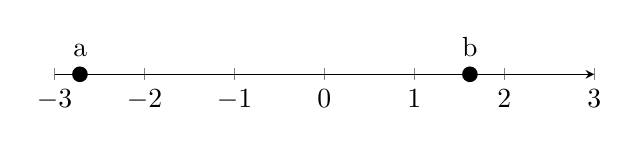
\begin{tikzpicture}
    \begin{axis}[
    % center the x axis
    axis x line=middle,
    % we don't need a y axis line ...
    axis y line=none,
    % ... and thus there is no need for much `height' of the axis
    height=100pt,
    % but `height' also changes `width' which is restored here
    width=\axisdefaultwidth,
    xmin=-3,
    xmax=3,
    ]
    \addplot[color=blue] coordinates {(-2.718,0)};
    \addplot[color=blue] coordinates {(1.618,0)};
    \node[label={above:{a}}, circle, fill, inner sep=2pt] at (axis cs:-2.718,0) {};
    \node[label={above:{b}}, circle, fill, inner sep=2pt] at (axis cs:1.618,0) {};
    \end{axis}
\end{tikzpicture}
	\caption{Numbers on the real line. In this example, we see that $a < b$ since $a$ is to the left of $b$.}
	\label{fig:real-line}
\end{figure*}

However, as we start working with more abstract mathematical objects, it becomes harder to define a notion of order based on spacial position.

Imagine that we have two infinite-dimensional arrays $(a_n)_{n=1}^\infty$ and $(b_n)_{n=1}^\infty$ of positive real numbers. As we have seen, there is no clear way to use $<$ to compare which has higher-order, so we may come up with a definition that *makes sense*. One such way is to define the hierarchy in terms of *growth*. Roughly speaking, we may want to come up with a definition that states that $a$ is of lesser order than $b$ if $b$ grows more quickly than $a$. A way to think about growth is to ask whether $a$ can *catch-up* $b$. If $a$ can eventually catch $b$ and stay *above* $b$, then $a$ grows more quickly than $b$ and we define $a$ to be of higher order (a more powerful series!). If, on the contrary, $a$ can never catch up $b$ it means that every value $a_n$ will be below $b$.

Consider the series $(a_n)_{n=1}^\infty = \{n^2 \vert n\in\mathbb{N}\}$ and $(b_n)_{n=1}^\infty = \{\texttt{fibo}(n) \vert n\in\mathbb{N}\}$, where $\texttt{fibo(n)}$ is a function that returns the $n$-th element of the Fibonacci sequence. (figure \ref{fig:growth-1}). For $n \leq 11$, $a_n \geq b_n$. However, at $n=12$, $a_{12} = b_{12}$ and, for $n\geq 13$ $a_n < b_n$.

\begin{figure*}[h!]
	\centering
	\scalebox{0.5}{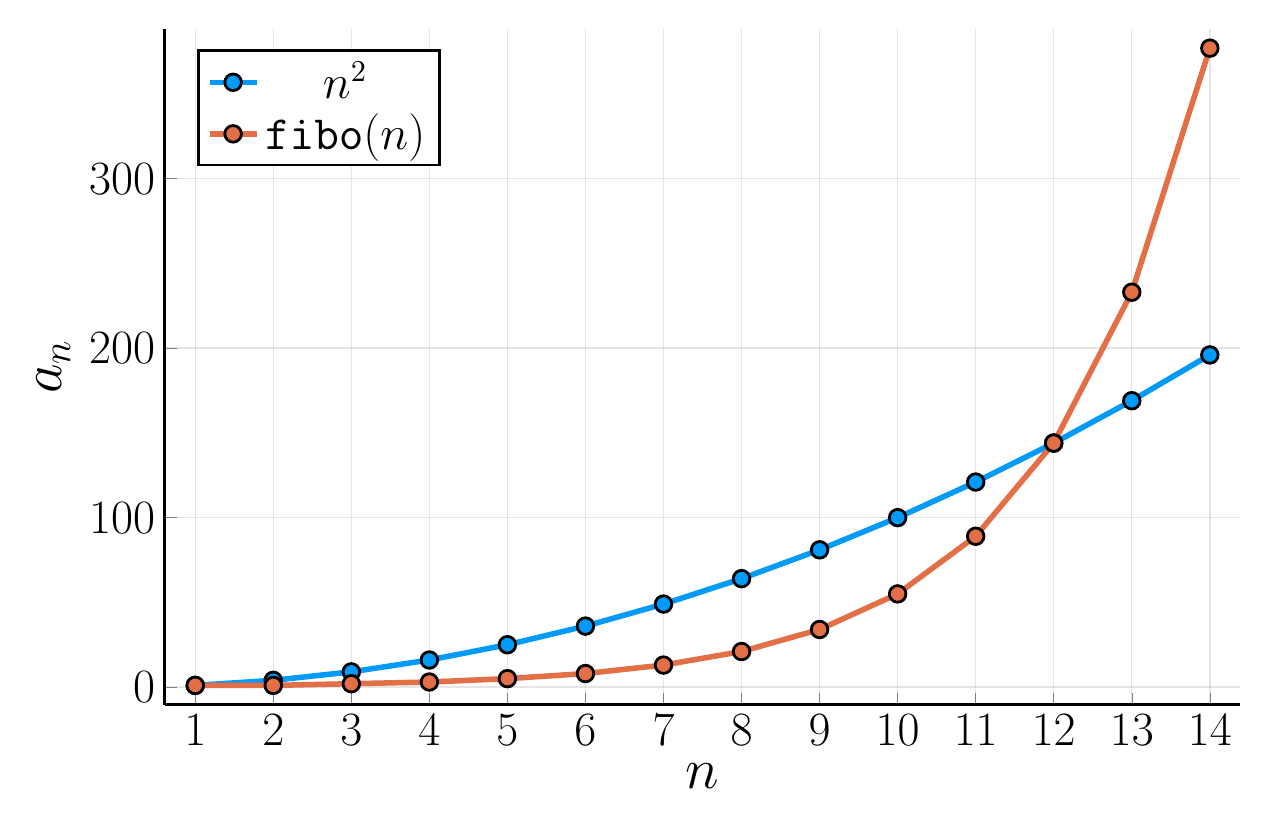
\begin{tikzpicture}[]
\begin{axis}[
  height = {101.6mm},
  legend pos = {north west},
  ylabel = {$a_n$},
  xmin = {0.61},
  xmax = {14.39},
  ymax = {388.28},
  xlabel = {$n$},
  unbounded coords=jump,scaled x ticks = false,xlabel style = {font = {\fontsize{22 pt}{28.6 pt}\selectfont}, color = {rgb,1:red,0.00000000;green,0.00000000;blue,0.00000000}, draw opacity = 1.0, rotate = 0.0},xmajorgrids = true,xtick = {1.0,2.0,3.0,4.0,5.0,6.0,7.0,8.0,9.0,10.0,11.0,12.0,13.0,14.0},xticklabels = {$1$,$2$,$3$,$4$,$5$,$6$,$7$,$8$,$9$,$10$,$11$,$12$,$13$,$14$},xtick align = inside,xticklabel style = {font = {\fontsize{16 pt}{20.8 pt}\selectfont}, color = {rgb,1:red,0.00000000;green,0.00000000;blue,0.00000000}, draw opacity = 1.0, rotate = 0.0},x grid style = {color = {rgb,1:red,0.00000000;green,0.00000000;blue,0.00000000},
draw opacity = 0.1,
line width = 0.5,
solid},axis x line* = left,x axis line style = {color = {rgb,1:red,0.00000000;green,0.00000000;blue,0.00000000},
draw opacity = 1.0,
line width = 1,
solid},scaled y ticks = false,ylabel style = {font = {\fontsize{22 pt}{28.6 pt}\selectfont}, color = {rgb,1:red,0.00000000;green,0.00000000;blue,0.00000000}, draw opacity = 1.0, rotate = 0.0},ymajorgrids = true,ytick = {0.0,100.0,200.0,300.0},yticklabels = {$0$,$100$,$200$,$300$},ytick align = inside,yticklabel style = {font = {\fontsize{16 pt}{20.8 pt}\selectfont}, color = {rgb,1:red,0.00000000;green,0.00000000;blue,0.00000000}, draw opacity = 1.0, rotate = 0.0},y grid style = {color = {rgb,1:red,0.00000000;green,0.00000000;blue,0.00000000},
draw opacity = 0.1,
line width = 0.5,
solid},axis y line* = left,y axis line style = {color = {rgb,1:red,0.00000000;green,0.00000000;blue,0.00000000},
draw opacity = 1.0,
line width = 1,
solid},    xshift = 0.0mm,
    yshift = 0.0mm,
    axis background/.style={fill={rgb,1:red,1.00000000;green,1.00000000;blue,1.00000000}}
,legend style = {color = {rgb,1:red,0.00000000;green,0.00000000;blue,0.00000000},
draw opacity = 1.0,
line width = 1,
solid,fill = {rgb,1:red,1.00000000;green,1.00000000;blue,1.00000000},fill opacity = 1.0,text opacity = 1.0,font = {\fontsize{16 pt}{20.8 pt}\selectfont}},colorbar style={title=},
  ymin = {-10.28},
  width = {152.4mm}
]

\addplot+[
  color = {rgb,1:red,0.00000000;green,0.60560316;blue,0.97868012},
draw opacity = 1.0,
line width = 2,
solid,mark = *,
mark size = 3.0,
mark options = {
            color = {rgb,1:red,0.00000000;green,0.00000000;blue,0.00000000}, draw opacity = 1.0,
            fill = {rgb,1:red,0.00000000;green,0.60560316;blue,0.97868012}, fill opacity = 1.0,
            line width = 1,
            rotate = 0,
            solid
        }
] coordinates {
  (1.0, 1.0)
  (2.0, 4.0)
  (3.0, 9.0)
  (4.0, 16.0)
  (5.0, 25.0)
  (6.0, 36.0)
  (7.0, 49.0)
  (8.0, 64.0)
  (9.0, 81.0)
  (10.0, 100.0)
  (11.0, 121.0)
  (12.0, 144.0)
  (13.0, 169.0)
  (14.0, 196.0)
};

\addplot+[
  color = {rgb,1:red,0.88887350;green,0.43564919;blue,0.27812294},
draw opacity = 1.0,
line width = 2,
solid,mark = *,
mark size = 3.0,
mark options = {
            color = {rgb,1:red,0.00000000;green,0.00000000;blue,0.00000000}, draw opacity = 1.0,
            fill = {rgb,1:red,0.88887350;green,0.43564919;blue,0.27812294}, fill opacity = 1.0,
            line width = 1,
            rotate = 0,
            solid
        }
] coordinates {
  (1.0, 1.0)
  (2.0, 1.0)
  (3.0, 2.0)
  (4.0, 3.0)
  (5.0, 5.0)
  (6.0, 8.0)
  (7.0, 13.0)
  (8.0, 21.0)
  (9.0, 34.0)
  (10.0, 55.0)
  (11.0, 89.0)
  (12.0, 144.0)
  (13.0, 233.0)
  (14.0, 377.0)
};

\legend{{}{$n^2$}, {}{$\texttt{fibo}(n)$}}
\end{axis}

\end{tikzpicture}

}
	\caption{Plot of two series}
	\label{fig:growth-1}
\end{figure*}

In fact, taking a close look at our example, we can see that the relative difference between $a_n$ and $b_n$ (defined as $a_n / b_n$) growths fast and reaches a peak at $n=4$. After this peak, $b_n$ starts growing faster and eventually reaching up, as shown in figure \ref{fig:relative-growth}.

\begin{figure*}[h!]
	\centering
	\scalebox{0.5}{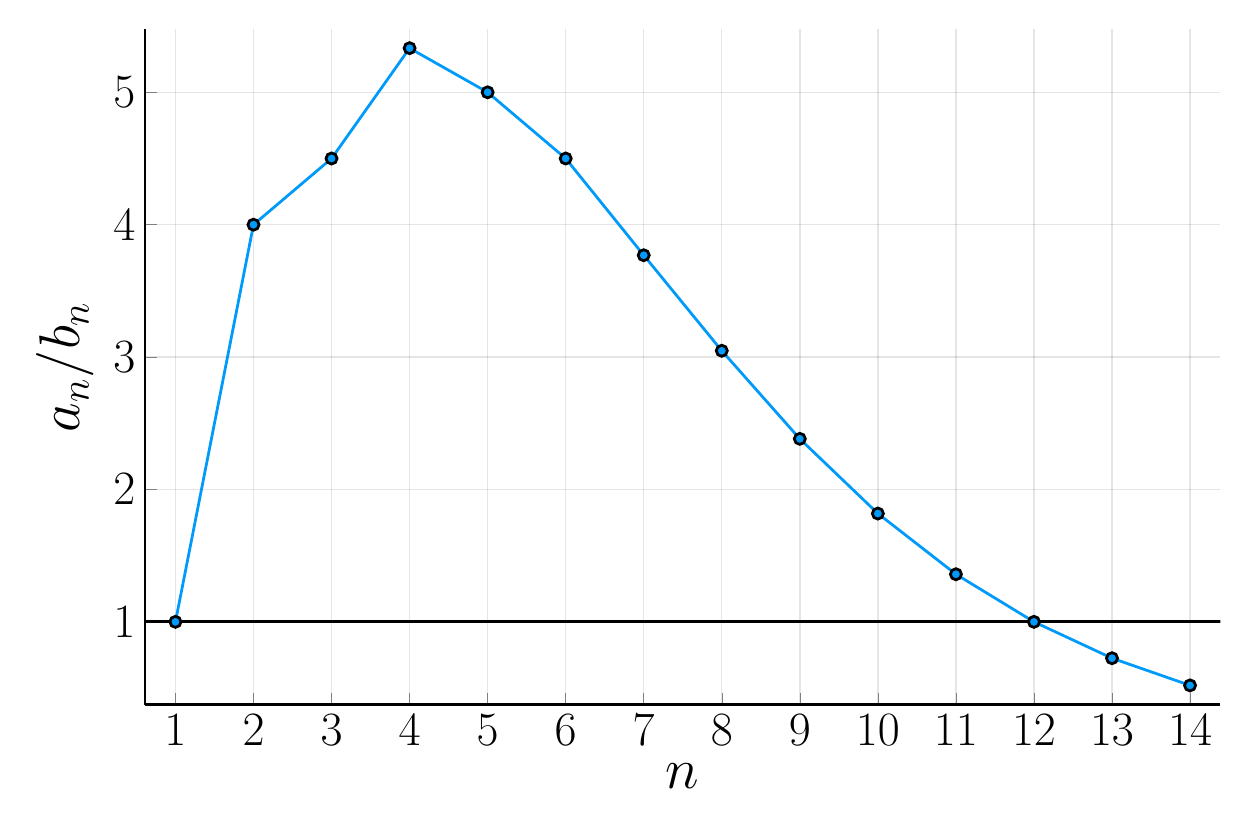
\begin{tikzpicture}[]
\begin{axis}[
  height = {101.6mm},
  ylabel = {$a_n / b_n$},
  xmin = {0.61},
  xmax = {14.39},
  ymax = {5.477736516357206},
  xlabel = {$n$},
  unbounded coords=jump,scaled x ticks = false,xlabel style = {font = {\fontsize{22 pt}{28.6 pt}\selectfont}, color = {rgb,1:red,0.00000000;green,0.00000000;blue,0.00000000}, draw opacity = 1.0, rotate = 0.0},xmajorgrids = true,xtick = {1.0,2.0,3.0,4.0,5.0,6.0,7.0,8.0,9.0,10.0,11.0,12.0,13.0,14.0},xticklabels = {$1$,$2$,$3$,$4$,$5$,$6$,$7$,$8$,$9$,$10$,$11$,$12$,$13$,$14$},xtick align = inside,xticklabel style = {font = {\fontsize{16 pt}{20.8 pt}\selectfont}, color = {rgb,1:red,0.00000000;green,0.00000000;blue,0.00000000}, draw opacity = 1.0, rotate = 0.0},x grid style = {color = {rgb,1:red,0.00000000;green,0.00000000;blue,0.00000000},
draw opacity = 0.1,
line width = 0.5,
solid},axis x line* = left,x axis line style = {color = {rgb,1:red,0.00000000;green,0.00000000;blue,0.00000000},
draw opacity = 1.0,
line width = 1,
solid},scaled y ticks = false,ylabel style = {font = {\fontsize{22 pt}{28.6 pt}\selectfont}, color = {rgb,1:red,0.00000000;green,0.00000000;blue,0.00000000}, draw opacity = 1.0, rotate = 0.0},ymajorgrids = true,ytick = {1.0,2.0,3.0,4.0,5.0},yticklabels = {$1$,$2$,$3$,$4$,$5$},ytick align = inside,yticklabel style = {font = {\fontsize{16 pt}{20.8 pt}\selectfont}, color = {rgb,1:red,0.00000000;green,0.00000000;blue,0.00000000}, draw opacity = 1.0, rotate = 0.0},y grid style = {color = {rgb,1:red,0.00000000;green,0.00000000;blue,0.00000000},
draw opacity = 0.1,
line width = 0.5,
solid},axis y line* = left,y axis line style = {color = {rgb,1:red,0.00000000;green,0.00000000;blue,0.00000000},
draw opacity = 1.0,
line width = 1,
solid},    xshift = 0.0mm,
    yshift = 0.0mm,
    axis background/.style={fill={rgb,1:red,1.00000000;green,1.00000000;blue,1.00000000}}
,legend style = {color = {rgb,1:red,0.00000000;green,0.00000000;blue,0.00000000},
draw opacity = 1.0,
line width = 1,
solid,fill = {rgb,1:red,1.00000000;green,1.00000000;blue,1.00000000},fill opacity = 1.0,text opacity = 1.0,font = {\fontsize{16 pt}{20.8 pt}\selectfont}},colorbar style={title=},
  ymin = {0.37549071618037133},
  width = {152.4mm}
]

\addplot+[
  color = {rgb,1:red,0.00000000;green,0.60560316;blue,0.97868012},
draw opacity = 1.0,
line width = 1,
solid,mark = *,
mark size = 2.0,
mark options = {
            color = {rgb,1:red,0.00000000;green,0.00000000;blue,0.00000000}, draw opacity = 1.0,
            fill = {rgb,1:red,0.00000000;green,0.60560316;blue,0.97868012}, fill opacity = 1.0,
            line width = 1,
            rotate = 0,
            solid
        },forget plot
] coordinates {
  (1.0, 1.0)
  (2.0, 4.0)
  (3.0, 4.5)
  (4.0, 5.333333333333333)
  (5.0, 5.0)
  (6.0, 4.5)
  (7.0, 3.769230769230769)
  (8.0, 3.0476190476190474)
  (9.0, 2.3823529411764706)
  (10.0, 1.8181818181818181)
  (11.0, 1.3595505617977528)
  (12.0, 1.0)
  (13.0, 0.7253218884120172)
  (14.0, 0.519893899204244)
};

\addplot+[
  color = {rgb,1:red,0.00000000;green,0.00000000;blue,0.00000000},
draw opacity = 1.0,
line width = 1,
solid,mark = none,
mark size = 2.0,
mark options = {
            color = {rgb,1:red,0.00000000;green,0.00000000;blue,0.00000000}, draw opacity = 1.0,
            fill = {rgb,1:red,0.00000000;green,0.00000000;blue,0.00000000}, fill opacity = 1.0,
            line width = 1,
            rotate = 0,
            solid
        },forget plot
] coordinates {
  (-13.170000000000002, 1.0)
  (28.17, 1.0)
};

\end{axis}

\end{tikzpicture}

}
	\caption{Plot of two series}
	\label{fig:relative-growth}
\end{figure*}

At it maximum value, $an$ is around 5 times greater than $bn$! What this means is that, since the relative difference between $an$ and $bn$ is bounded above (it is never greater than 5x), if we multiply each entry of $bn$ by 5.333, then every element of $b$ will always be less than or equal to $a$. In other words, $a$ can never catch $b$ if the relative distance is finite, that is to say, there exists some constant $C$ such that for every $n=1\ldots$, $a_n \leq C \cdot b_n$. Armed with this intuition, we can formally define the relationship $\prec$ between two series $(a_n)_n$ and $(b_n)_n$ as follows:


\begin{figure*}[h!]
	\centering
	\scalebox{0.5}{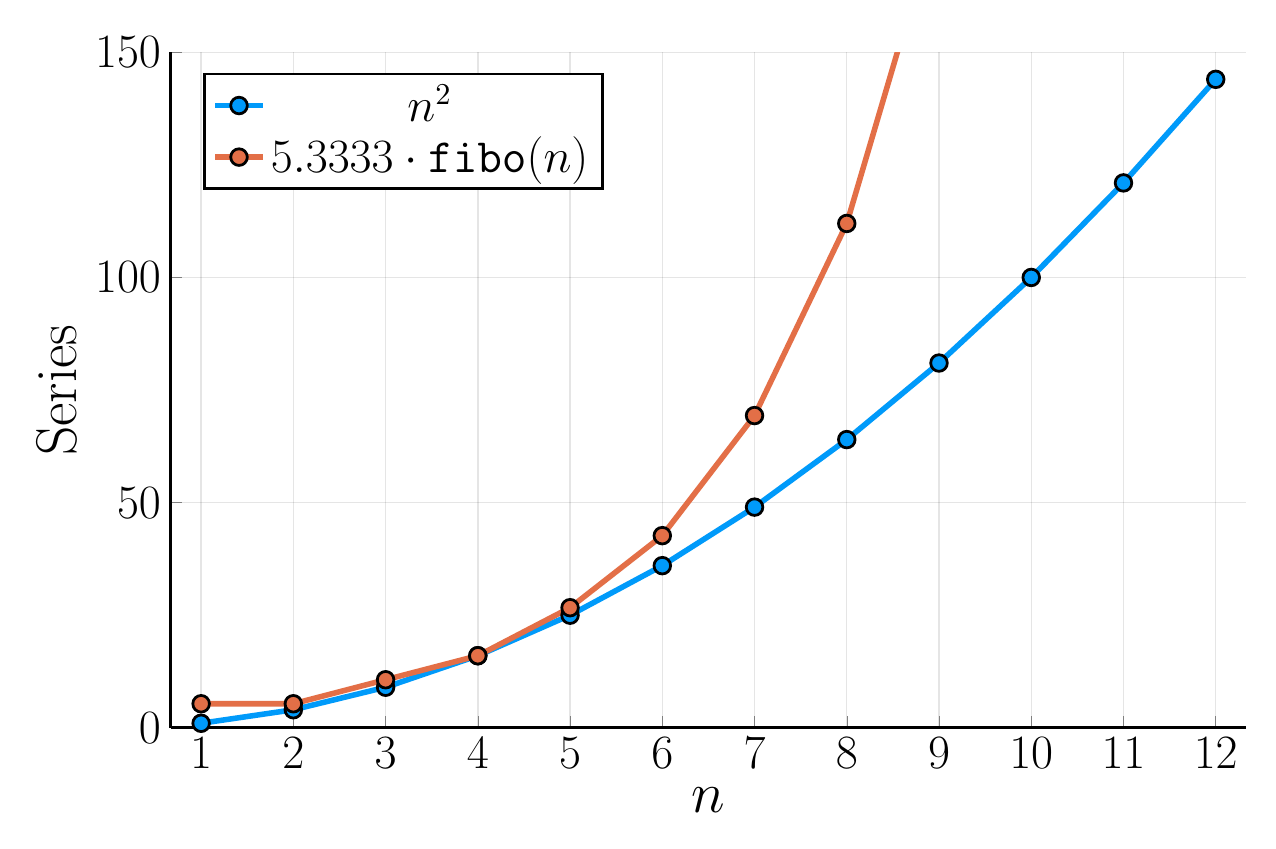
\begin{tikzpicture}[]
\begin{axis}[
  height = {101.6mm},
  legend pos = {north west},
  ylabel = {Series},
  xmin = {0.67},
  xmax = {12.33},
  ymax = {150},
  xlabel = {$n$},
  unbounded coords=jump,scaled x ticks = false,xlabel style = {font = {\fontsize{22 pt}{28.6 pt}\selectfont}, color = {rgb,1:red,0.00000000;green,0.00000000;blue,0.00000000}, draw opacity = 1.0, rotate = 0.0},xmajorgrids = true,xtick = {1.0,2.0,3.0,4.0,5.0,6.0,7.0,8.0,9.0,10.0,11.0,12.0},xticklabels = {$1$,$2$,$3$,$4$,$5$,$6$,$7$,$8$,$9$,$10$,$11$,$12$},xtick align = inside,xticklabel style = {font = {\fontsize{16 pt}{20.8 pt}\selectfont}, color = {rgb,1:red,0.00000000;green,0.00000000;blue,0.00000000}, draw opacity = 1.0, rotate = 0.0},x grid style = {color = {rgb,1:red,0.00000000;green,0.00000000;blue,0.00000000},
draw opacity = 0.1,
line width = 0.5,
solid},axis x line* = left,x axis line style = {color = {rgb,1:red,0.00000000;green,0.00000000;blue,0.00000000},
draw opacity = 1.0,
line width = 1,
solid},scaled y ticks = false,ylabel style = {font = {\fontsize{22 pt}{28.6 pt}\selectfont}, color = {rgb,1:red,0.00000000;green,0.00000000;blue,0.00000000}, draw opacity = 1.0, rotate = 0.0},ymajorgrids = true,ytick = {0.0,50.0,100.0,150.0},yticklabels = {$0$,$50$,$100$,$150$},ytick align = inside,yticklabel style = {font = {\fontsize{16 pt}{20.8 pt}\selectfont}, color = {rgb,1:red,0.00000000;green,0.00000000;blue,0.00000000}, draw opacity = 1.0, rotate = 0.0},y grid style = {color = {rgb,1:red,0.00000000;green,0.00000000;blue,0.00000000},
draw opacity = 0.1,
line width = 0.5,
solid},axis y line* = left,y axis line style = {color = {rgb,1:red,0.00000000;green,0.00000000;blue,0.00000000},
draw opacity = 1.0,
line width = 1,
solid},    xshift = 0.0mm,
    yshift = 0.0mm,
    axis background/.style={fill={rgb,1:red,1.00000000;green,1.00000000;blue,1.00000000}}
,legend style = {color = {rgb,1:red,0.00000000;green,0.00000000;blue,0.00000000},
draw opacity = 1.0,
line width = 1,
solid,fill = {rgb,1:red,1.00000000;green,1.00000000;blue,1.00000000},fill opacity = 1.0,text opacity = 1.0,font = {\fontsize{16 pt}{20.8 pt}\selectfont}},colorbar style={title=},
  ymin = {0},
  width = {152.4mm}
]

\addplot+[
  color = {rgb,1:red,0.00000000;green,0.60560316;blue,0.97868012},
draw opacity = 1.0,
line width = 2,
solid,mark = *,
mark size = 3.0,
mark options = {
            color = {rgb,1:red,0.00000000;green,0.00000000;blue,0.00000000}, draw opacity = 1.0,
            fill = {rgb,1:red,0.00000000;green,0.60560316;blue,0.97868012}, fill opacity = 1.0,
            line width = 1,
            rotate = 0,
            solid
        }
] coordinates {
  (1.0, 1.0)
  (2.0, 4.0)
  (3.0, 9.0)
  (4.0, 16.0)
  (5.0, 25.0)
  (6.0, 36.0)
  (7.0, 49.0)
  (8.0, 64.0)
  (9.0, 81.0)
  (10.0, 100.0)
  (11.0, 121.0)
  (12.0, 144.0)
};

\addplot+[
  color = {rgb,1:red,0.88887350;green,0.43564919;blue,0.27812294},
draw opacity = 1.0,
line width = 2,
solid,mark = *,
mark size = 3.0,
mark options = {
            color = {rgb,1:red,0.00000000;green,0.00000000;blue,0.00000000}, draw opacity = 1.0,
            fill = {rgb,1:red,0.88887350;green,0.43564919;blue,0.27812294}, fill opacity = 1.0,
            line width = 1,
            rotate = 0,
            solid
        }
] coordinates {
  (1.0, 5.333)
  (2.0, 5.333)
  (3.0, 10.666)
  (4.0, 15.999)
  (5.0, 26.665)
  (6.0, 42.664)
  (7.0, 69.32900000000001)
  (8.0, 111.99300000000001)
  (9.0, 181.322)
  (10.0, 293.315)
  (11.0, 474.637)
  (12.0, 767.952)
};

\legend{{}{$n^2$}, {}{$5.3333 \cdot \texttt{fibo}(n)$}}
\end{axis}

\end{tikzpicture}

}
	\caption{Plot of two series}
	\label{fig:growth-2}
\end{figure*}


\begin{definition}
	Let $(a_n)_{n=1}^\infty$, $(b_n)_{n=1}^\infty$ be sequences of positive real numbers. We say that $(a_n)_{n=1}^\infty \prec (b_n)_{n=1}^\infty$. If there exists $C\in\mathbb{R}^{+}$ such that for every $n\in\mathbb{N}. a_n \leq C\cdot b_n$
\end{definition}

\subsection*{Belief Propagation}
\subsubsection*{Inference and graphical models}
The computation of marginal probabilities of graphical models is known as inference. The Belief Propagation (BP) algorithm is used to efficiently make inference over graphical models.

Three main kinds of graphical models are Bayesian Networks, pairwise Markov Random Fields (MRF), and Factor Graphs. Each of these represent the joint probability of a set of random variables in different graphical ways. There are different methods to perform inference over each of these graphs, but they are all variants of the BP algorithm.


Bayesian Networks are directed graphs for modeling conditional relationships by assuming that the joint distribution of a set of random variables can be described as

\begin{equation*}
	p(x_1, \ldots, x_N) = \prod_{n=1}^Np(x_n\vert \text{Pa}(x_n))
\end{equation*}

where $\text{Pa}(x_n)$ denote the set of nodes that have a \textit{causal} effect on $x_n$.

Pairwise Markov Random Fields, on the other hand, are undirected graphs with an application for computer vision problems. Their joint distribution can be described as a function of neighboring unobserved nodes and pairs of observed and unobserved nodes.

\begin{equation*}
	p({\bf x}, {\bf y}) = \frac{1}{Z}\prod_{n,m}\psi_{nm}(x_n, x_m)\prod_{n}\phi(x_n, y_n)
\end{equation*}

Finally, Tanner Graphs have their origins in an application for decoding of error-correcting codes. Their graphical representation is known as a Factor Graphs with joint probability defined as

\begin{equation*}
	p({\bf x}) = \frac{1}{Z}\prod_{m=1}^M \psi_m(x_m)
\end{equation*}

All three graphical models are equivalent. That is, one can represent a pairwise MRF or Bayesian network into equivalent factor graphs or vice-versa.

The Belief Propagation has different variants depending on the type of graph one choses to work with. Therefore, by deriving the BP algorithm on a pairwise MRF one can generalize the results to the other types of graphical models.

\subsubsection*{Standard Belief Propagation}
The main idea behind the Belief Propagation algorithm for pairwise MRFs is the introduction of messages from one node to the other to efficiently make inference on an unobserved node $x_n$, which results in obtaining the ``belief'' of the node $x_n$, denoted as $b_n(x_n)$.

These ``messages'' introduced by the BP model ameliorate the need to compute in exponential time the marginal probability of a node $x_n$:

\begin{equation*}
	p(x_n) = \sum_{x_m \vert m \neq n} p(x_m),
\end{equation*}

but insted compute this value in terms of the neighboring nodes of $x_n$:

\begin{equation*}
	p(x_n) \propto \phi_n(x_n, y_n) \prod_{j \in N(x_n)} m_{j,n}(x_n)
\end{equation*}

The messages in the BP algorithm are computed recursively until all messages are known. This is done by computing a message as

\begin{equation*}
	m_{ij}(x_j) \leftarrow \sum_{x_i} \phi(x_i) \psi_{ij}(x_i, x_j) \prod_{k \in N(i) \backslash j} m_{ki}(x_i)
\end{equation*}

In practice, one starts by computing the messages at the edges of the graph and propagate the messages if necessary.
\end{document}